%\definition
A segment tree is a static binary search tree for a given set of
coordinates. The set of coordinates is defined by the endpoints
of the input data intervals. Any two adjacent coordinates
build an elementary interval. Every leaf corresponds to an
elementary interval.
Inner vertices
correspond to the union of the subtree intervals of the vertex.
Each vertex or leaf $v$ contains a sublayer type (or a
list, if it is one-dimensional) that will contain all intervals $I$, such that
$I$  contains the interval of vertex $v$ but not the interval
of the parent vertex of $v$.

A $d$-dimensional segment tree can be used to solve the following problems:
\begin{itemize}
\item Determine all $d$-dimensional intervals that contain a
  $d$-dimensional point. This query type is called ``inverse
  range query''.
  \item Determine all $d$-dimensional intervals that enclose a
    given $d$-dimensional interval
    (\ccStyle{enclosing\_query}).
  \item Determine all $d$-dimensional intervals that partially overlap or are
    contained in a given $d$-dimensional interval (\ccStyle{window\_query}).
\end{itemize}

\begin{ccTexOnly}
In Figure~\ref{User:fig:segment2.eps} an example of a one-dimensional segment 
tree is given. Figure~\ref{User:fig:d-segment.eps} shows a two-dimensional
segment tree.
\end{ccTexOnly}

\begin{ccHtmlOnly}
An example of a one-dimensional segment tree and an example
of a two-dimensional segment tree are shown below.
\end{ccHtmlOnly}

\begin{ccTexOnly}
\begin{figure}[htbp]
\centering
\begin{minipage}{11cm}
    \begin{center}
    \includegraphics[width=8cm,clip]{segment2.eps}
    \end{center}
\caption{\label{User:fig:segment2.eps}A one-dimensional segment
  tree. The segments and the corresponding elementary intervals
  are shown below the tree. The arcs from the nodes point to
  their subsets.}
\vspace{2\baselineskip}
\end{minipage}
\hspace*{1em}
\begin{minipage}{11cm}
    \begin{center}
    \includegraphics[width=8cm,clip]{d-segment.eps}
    \end{center}
\caption{\label{User:fig:d-segment.eps}A two-dimensional segment
  tree. The first layer of the tree is built according to the
  elementary intervals of the first dimension. Each
  sublayer tree of a vertex $v$ is a segment tree according to
  the  second dimension of all data items of $v$.}

\end{minipage}
\end{figure}
\end{ccTexOnly}

\begin{ccHtmlOnly}
    <!2><TABLE BORDER=0 CELLSPACING=2 CELLPADDING=0 WIDTH=650>
        <TR>
    <A NAME="User:fig:segment2.eps"></A>
    <TD ALIGN=LEFT VALIGN=TOP WIDTH=50% NOWRAP COLSPAN=2>
    <img border=0 src="./segment2.gif" alt="A one-dimensional segment
tree">
    </TD>
    <A NAME="User:fig:d-segment.eps"></A>
    <TD ALIGN=LEFT VALIGN=TOP WIDTH=50%><img border=0
src="./d-segment.gif" alt="A d-dimensional segment tree">
      </TD></TR></TABLE>

        <!2><TABLE BORDER=0 CELLSPACING=2 CELLPADDING=0 WIDTH=650>
        <TR><TD ALIGN=LEFT VALIGN=TOP WIDTH=50%  COLSPAN=2>
A one-dimensional segment
  tree. The segments and the corresponding elementary intervals
  are shown below the tree. The arcs from the nodes point to
  their subsets.
 </TD><TD ALIGN=LEFT VALIGN=TOP WIDTH=45%>
A two-dimensional segment
  tree. The first layer of the tree is built according to the
  elementary intervals of the first dimension. Each
  sublayer tree of a vertex  <MATH>v</MATH> is a segment tree according to
  the  second dimension of all data items of  <MATH>v</MATH>.
 </TD></TR>
        </TABLE><!2>
\end{ccHtmlOnly}

%The tree can be built in  ${\cal O}(n\log^{d} n)$ time and
%needs  ${\cal O}(n\log^{d} n)$ space.
%The  processing time for inverse range
%queries in an $d$-dimensional segment tree is ${\cal O}(\log^d n
%+k)$ time, where $n$ is the total number of intervals and $k$ is
%the number of reported intervals.
The tree can be built in  $O(n\log^{d} n)$ time and
needs  $O(n\log^{d} n)$ space.
The  processing time for inverse range
queries in an $d$-dimensional segment tree is $O(\log^d n
+k)$ time, where $n$ is the total number of intervals and $k$ is
the number of reported intervals.

One possible application of a two-dimensional segment tree is the
following. Given a set of convex polygons in two-dimensional
space (CGAL::Polygon\_2), we want to determine all polygons
that intersect a given rectangular query window. Therefore, we define a
two-dimensional segment tree, where the two-dimensional interval of
a data item corresponds to the  bounding box of a polygon and the
value type corresponds to the polygon itself. The segment tree is created
with a sequence of all data items, and a window query is
performed. The polygons of the resulting data items are finally
tested independently for intersections.

